\documentclass[useAMS,usenatbib]{mn2e}
\usepackage{myaasmacros}
\usepackage{graphicx}
\usepackage{ulem}
\usepackage{color}
\usepackage{amsmath}

% Some definitions of things I always use here:
\def\ltsima{$\; \buildrel < \over \sim \;$}
\def\simlt{\lower.5ex\hbox{\ltsima}}   
\def\gtsima{$\; \buildrel > \over \sim \;$}
\def\simgt{\lower.5ex\hbox{\gtsima}}
\def\siglos{\sigma_{\text{LOS}}}
\def\siglosi{\sigma_{\text{LOS},i}}
\newcommand\bcite[1]{(\citeauthor{#1} \citeyear{#1})}

\newcommand{\changefont}[3]{
\fontfamily{#1} \fontseries{#2} \fontshape{#3} \selectfont}

\newcommand{\TODO}[1]{\textsc{\textbf{\textcolor{red}{(TODO: #1)}}}}

% Some definitions for the priors:
\def\gprior{{\tt gprior}}
\def\cprior{{\tt cprior}}
\def\bprior{{\tt bprior}}
\def\lbprior{{\tt lbprior}}

%Some definitions for rhodm etc:
\def\vztwo{\overline{v_z^2}}
\def\vztwoi{\overline{v_{z,i}^2}}
\def\rhodisc{\rho_\mathrm{disc}(z)}
\def\rhodmext{\rho_\mathrm{dm,ext}}
\def\rhodm{\rho_\mathrm{dm}}
\def\rhoeff{\rho_\mathrm{dm}^\mathrm{eff}}
\def\nuobs{\nu_\mathrm{obs}(z)}
\def\tot{\mathrm{tot}}
\def\kpc{\mathrm{kpc}}

\title[Non-parametric method for mass modelling spherical systems]{Non-parametric method for mass modelling spherical systems}

\author[Steger]{P. Steger$^1$\thanks{E-mail: psteger@phys.ethz.ch}, D. von Rickenbach$^1$, J. I. Read$^{1,2}$\\
$^1$Institute for Astronomy, Department of Physics, ETH Z\"urich, Wolfgang-Pauli-Strasse 27, CH-8093 Z\"urich, Switzerland\\
$^2$Department of Physics, University of Surrey, Guildford, GU2 7XH, UK
}

\begin{document}

\maketitle

\begin{abstract}
We propose a new non-parametric method to determine the mass
distribution in spherical systems. A high dimensional parameter space
encoding tracer density, line of sight velocity dispersion and total
mass density is sampled with a MultiNest parameter space explorer.

Without assumptions on the functional form of any of these profiles,
we can reproduce liably the total mass density of mock dwarf galaxies,
and disentangle the degeneracy between dark matter density and tracer
velocity anisotropy.

We show early applications to observed dwarf galaxies, and point out
what data quality is required to detect cores of radius $r_c$.
\end{abstract}

\begin{keywords} galaxies: dwarf  -- galaxies: fundamental parameters  -- galaxies: kinematics and dynamics -- cosmology: dark matter
\end{keywords}

% input does not clear page, include does. could use newclude package and include*

\section{Introduction}\label{sec:introduction}


%%% Local Variables:
%%% mode: latex
%%% TeX-master: "Steger+_2014_OtherDwarfs"
%%% End:

\section{Method}\label{sec:method}
We employ the non-parametric mass modelling described in
\TODO{citep{Steger+2014}}:

The total mass density is given in bins by setting the density slope

\begin{equation}
n(r_j)=-{\rm d}\ln\rho(r)/{\rm d}\ln r|_{r=r_j}
\end{equation}
for $j ... N_{\rm bin}$ radial bins: $1\leq j\leq N_{\rm bin}$, and
interpolated linearly in between bin radii $r_{{\rm min},j}<r<r_{{\rm
    max},j}$.

The density then is given by
\begin{equation*}
    \rho(r) = \rho_{1/2}\cdot\exp\left[-\int_{\ln r_{1/2}}^{\ln r}n(s)\text{d}s\right],
\end{equation*}
with the density at half-light radius $\rho(r_{1/2})=\rho_{1/2}$, We
prescribe three buffer bins $n(r_j)$ for $j\in\{N_{\rm bin}+1,
N_{\rm bin}+2, N_{\rm bin}+3\}$ outside of the range where data is given to
enable sensible extrapolations towards high radii, and two additional slopes
$n_0 < 3, n_\infty>3$ for the asymptotic density slopes towards $r=0$ and
$r=\infty$, which are reached at half the smallest radius and $r_\infty=10r_{\rm
  max}$.


\subsection{Splitting Populations}\label{sec:metals}
Observations of the abundances of metals and chemical species in the
stellar atmospheres show that the ensemble of stars in a dwarf galaxy
or globular cluster can be split into populations.

An approach by \cite{WalkerPenarrubia2011} showed that if the
population of Fornax is split into two populations based on Magnesium
index and positions and LOS velocities assuming a Plummer sphere, and
each of their half-light radius and mass inside that radius are
determined, restrictions on the overall potential can be drawn. Using
this approach, they prefer a cored DM profile for Fornax.

For our data, we will use a splitting based on Magnesium index alone. This is
achieved by using a separate Markov Chain Monte Carlo method. The
overall Magnesium index distribution is represented by a sum of two
Gaussians with means $\mu_{1,2}$ and widths $\sigma_{1,2}$, and each
stellar tracer with Mg index $M$ is assigned a population based on
the likelihood of its metallicity belonging to said population. The
process is repeated to marginalize over the means and widths of the
metallicity distributions. A sample splitting result is shown in
fig. ~\ref{fig:pymcmetal}.

\begin{figure}
    \begin{center}
        %\hspace{-7mm}
        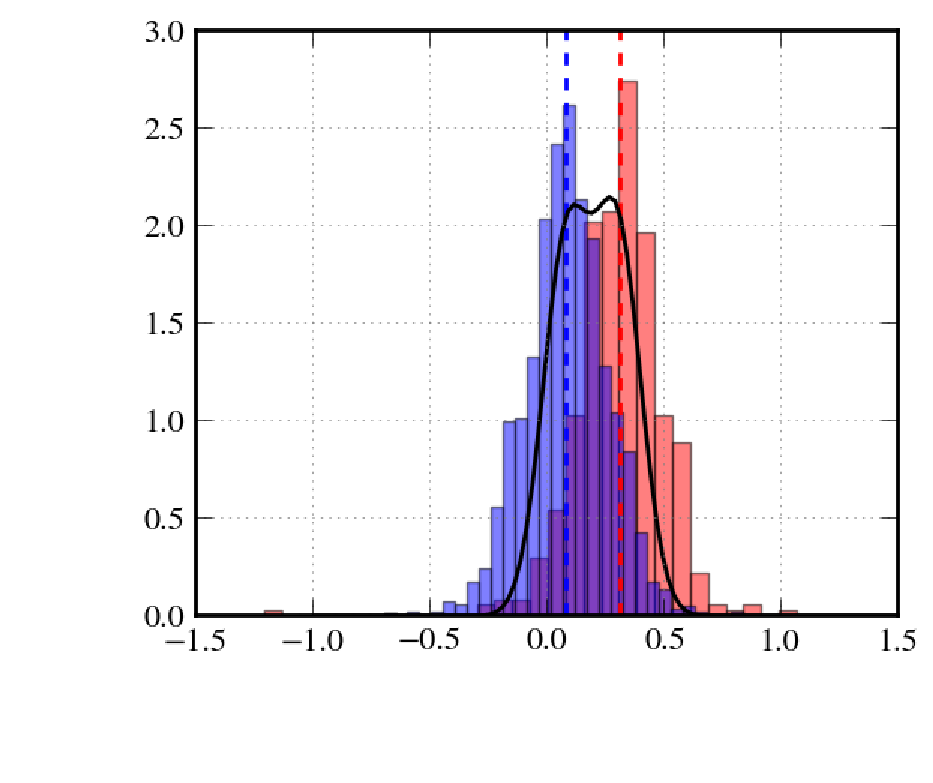
\includegraphics[width=0.5\textwidth]{fig/pymcmetals}
        \caption{Reconstruction of two populations from mock data. The
          underlying metallicity distributions are shown as red and
          blue histograms. The retrieved centers of the Gaussians are
          shown as vertical lines, and the reconstructed metallicity
          distribution is depicted as black line.}
        \label{fig:pymcmetal}
    \end{center}
\end{figure}

We restrict the method to Mg indices only, as the iron measurements in
\cite{WalkerPenarrubia2011} are not reliable enough, and a sizeable
fraction has no metallicity measurements.

\cite{WalkerPenarrubia2011} assume a Plummer-like profile for both
populations, which must be dropped in our non-parametric profile. We
additionally let drop the velocity information, and concentrate on
non-kinematic properties of the stars only. Foreground stars are
accounted for by weighting the probabilities of membership in each
population with the overall dSph probability of membership.

We first assume two populations, and from the pdf of the Mg indices,
we calculate the tracer density profiles for both populations. Each
star contributes to both populations, with a fraction given by its
probability of belonging to the chemical population $i$.

If we then see no significant difference between the half-light radii
distribution of all models with two populations, we conclude that
population splitting for that particular galaxy will not give us a
significant information gain in \GravImage\ .

If we on the other hand get a distinct peak in the pdf of the
half-light radii we know that there are two -- or possibly more --
distinct populations we can use for further analysis.

Optimally, we assign each star randomly in proportion to $f_i$ to
population $i$ for each step in the MultiNest procedure.


\subsection{Detailed Explanation}
In our test suite there are dwarf galaxies with different scale radii
and small differences in the mean of the metallicity for the two
populations of stars. In order to reproduce the underlying populations
we use an inset MCMC with assumptions that

\begin{enumerate}
\item Foreground stars are younger than most of the dSph member
  stars. Therefore, they show a high metallicity and can be removed
  from the dataset with a single cut in metallicity;
\item the remaining stellar components are divided into two
  populations;
\item the fraction of stars in population 1 is sampled in a uniform
  way in the range $[0,1]$;
\item both populations show a normal distribution in metallicity with
  an individual width;
\end{enumerate}

To test whether the assignment into populations is a valid one, we
want to check whether the population is in equilibrium with the
overall potential.

The routine then assigns each particle to one of the two populations,
based on its Mg metallicity. $75\pm4\%$ of all stars are assigned to
the correct underlying distribution on a mock dataset from the Gaia challenge. This
in turn changes the half-light radius by $110$pc and $-62$pc for
initial 390 pc, 730 pc half light radii. These changes are rather
high, but the two populations still show distinct half-light radii.

We explicitly assume two populations of stellar tracers in dwarf
galaxies, each with Gaussian distributions in metallicity with means
$\mu_1,\mu_2$. Without requiring a minimum distance $\delta
\mu=\mu_2-\mu_1$ between them, a representation with $\mu_1 \approx
\mu_2$ can be found. This model shows a higher $\chi^2$ than other
models and is thus disfavoured, but cannot be rejected from a
Kolmogorov-Smirnov test on a $p<0.05$ basis.

Here we show the influence of setting a prior minimal
$\delta\mu_{\min}$ on the goodness of fit, and the allowed range of
$\delta \mu$. We work on the metallicity distribution of one of the
mock dwarfs with cusped density profiles described earlier on, setting

\begin{equation} \mu_1\in[-1.0,2.0];\quad \delta \mu \in [
\delta\mu_{\min}, 5.0];\quad
\end{equation}

with $\delta\mu_{\min}$ varying from $0.0$ to $0.4$. We let the MCMC
run for a) 10k iterations with 8k burn-in/discarded models; b) 50k
iterations with 40k burn-in. From the accepted models, we compute the
mean Gaussian distributions and compare the corresponding overall
bimodal distribution to the actual metallicity distribution from the
data with a 2 component Kolmogorov-Smirnov test, and take the
two-tailed statistics $p_{\text KS}$ from 30 drawings. If $p_{\text
KS}>0.05$, then we cannot reject the hypothesis that the distributions
of the two samples are the same.

Results for varying the minimal distance between the two Gaussians
between $0.0$ and $0.4$ are shown in fig ~\ref{fig:kit}.

\begin{figure*}
    \begin{center} \hspace{-7mm}
        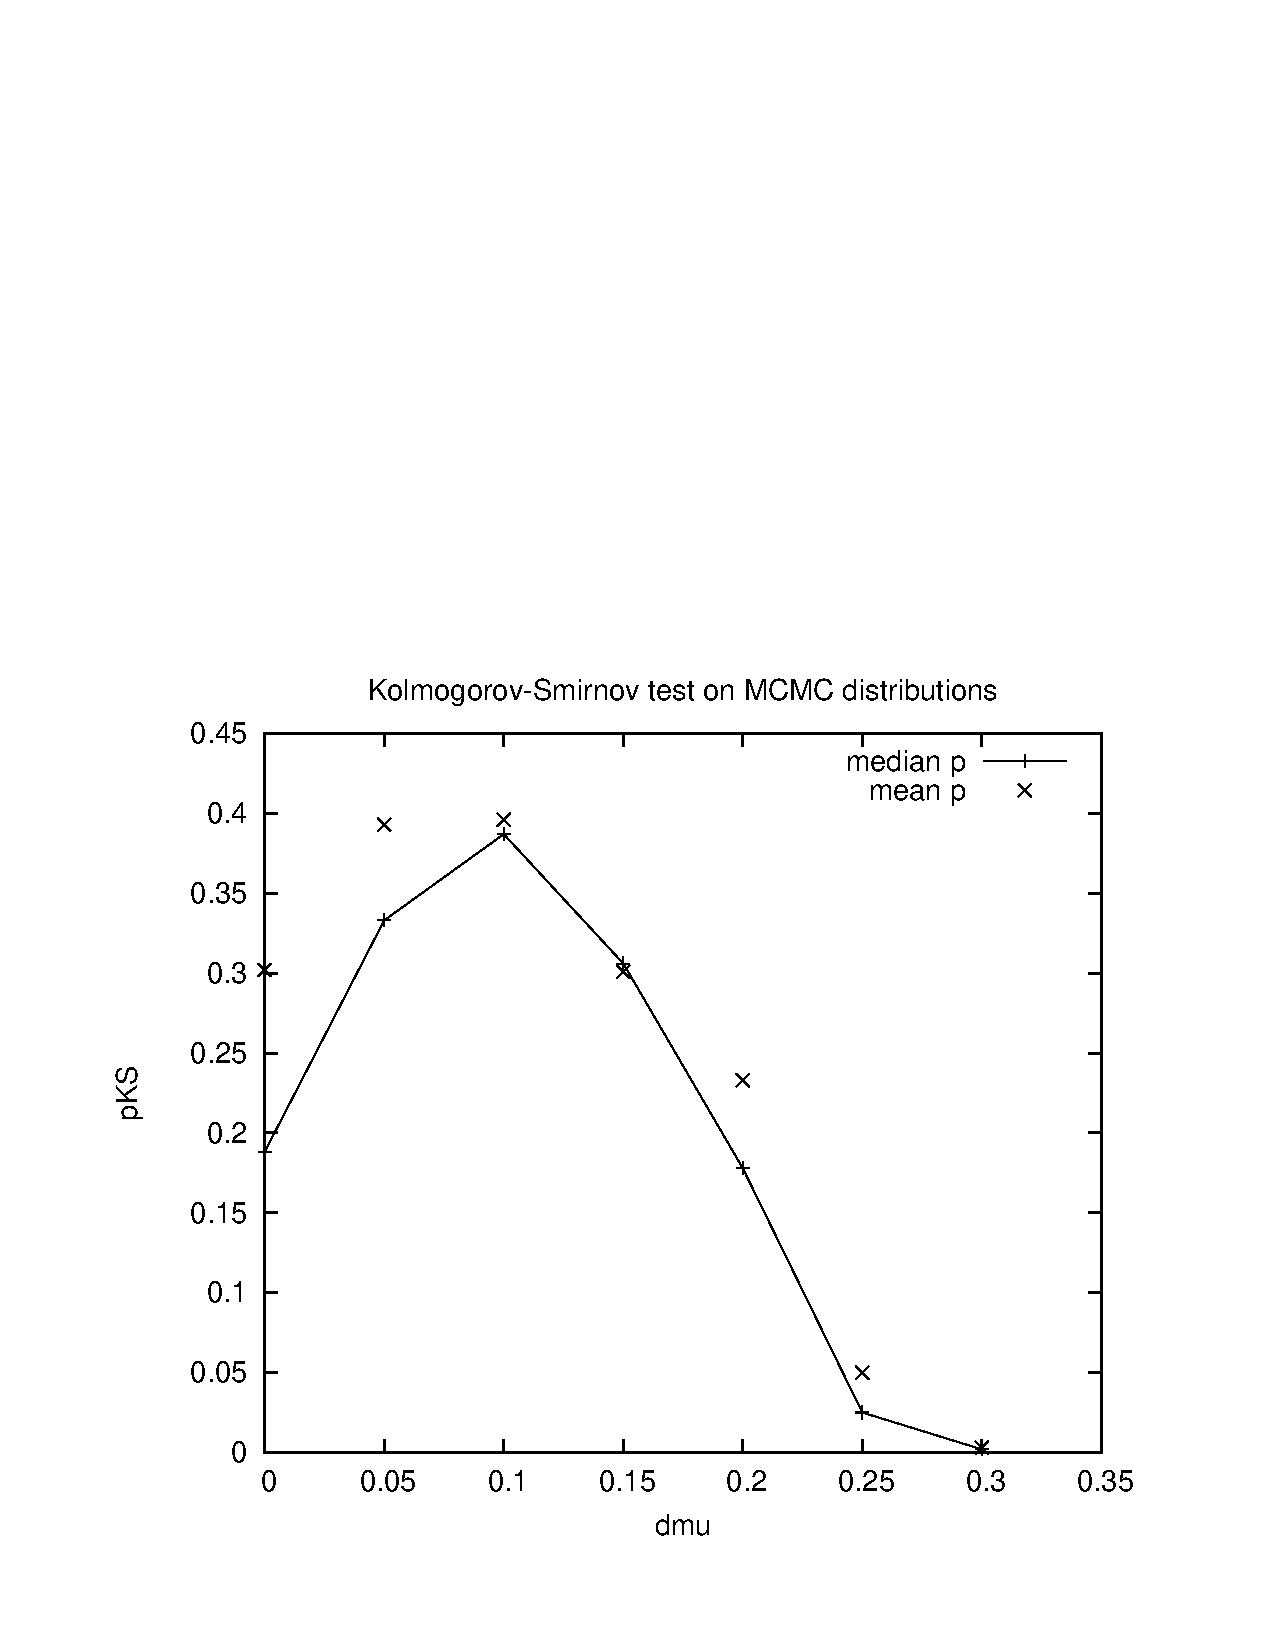
\includegraphics[width=0.5\textwidth]{fig/10kit.pdf}
        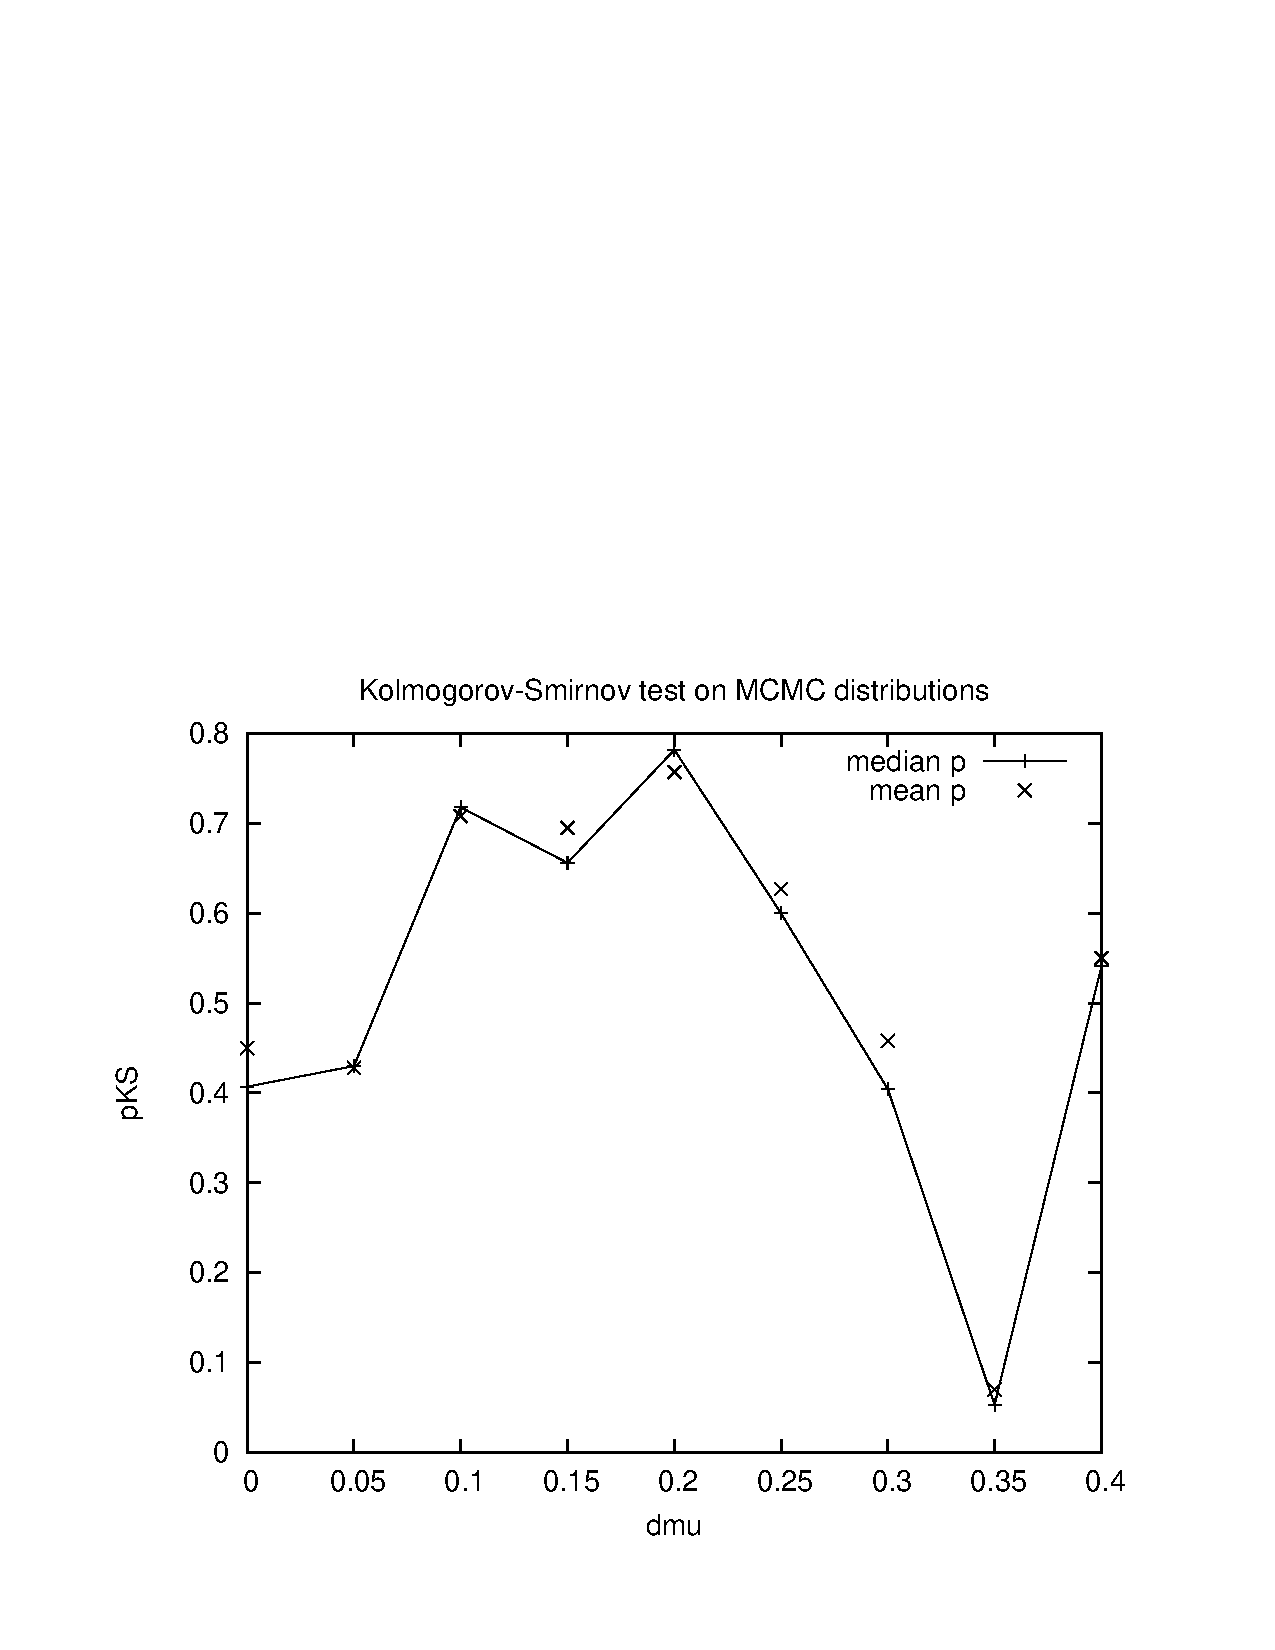
\includegraphics[width=0.5\textwidth]{fig/50kit.pdf}
        \caption{Kolmogorov-Smirnov test statistic $p_{\text KS}$ for
correspondance between models with $\delta\mu>\delta\mu_{\min}$ as
described in the text.}
        \label{fig:kit}
    \end{center}
\end{figure*}
All models with $p>0.05$ give a reasonable fit, with a maximum for 10k
iterations at around $\delta \mu = 0.1$. Models with $\delta \mu>0.2$
give no good fit anymore after 10k iterations.

The goodness of fit is enhanced if we take more iterations, so in the
plot for 50k iterations, there is a maximum $p=0.79$ compared to
$p=0.4$ from 10k iterations only. The whole curve is shifted to higher
$\delta \mu$ values. The models with $\delta \mu>0.3$ are
rejected. The restriction of $\delta \mu>0.4$ (last point to the
right) is well-fitting again, but this is due to the fact that the
fraction of particles for population 2 was found to be smaller than 10
percent, thus mainly fitting the metallicity distribution with one
Gaussian only, plus some skewing from an almost negligible stellar
component. Although this model cannot be rejected, it lies above the
rejected models at $\delta\mu_{\min}=0.4$. Furthermore, it does not
yield a second component with a scale length distinctly different from
the main component, rendering the additional gain from two components
obsolete. Thus, we will restrict the MCMC search of the population
fraction to the range $f\in[0.3,0.7]$.

\subsection{Baryonic Density Profiles}
Our Jeans-based method finds constraints on the overall mass density
profile

\begin{equation}
  \rho_{\rm tot} = \rho_{\rm DM}+\rho_{\rm bary}
\end{equation}
where $\rho_{\rm DM}$ is the dark matter density profile, and
$\rho_{\rm bary}$ is the baryonic density profile. As we are mostly
interested in the dark matter, we need to subtract the baryonic
contribution.

As the kinematic data we have is rather sparse -- not each star in the
dSph has its LOS velocity measured -- and misses other contributions
like gas, we subtract a photometrically defined baryonic density.

The errors on this density are rather small, thus we only use the
deprojected 3D photometric density profile for the subtraction,
without sampling over its errors, as is done for the kinematic tracer
population profiles.


%%% Local Variables:
%%% mode: latex
%%% TeX-master: "Steger+_2014_Fornax"
%%% End:

\section{Mock data}\label{sec:mocks}

We apply our method to a set of mock data,
consisting of multiple tracers moving in spherical
or triaxial potentials with radial or tangential
velocity anisotropy. All mock data are available
on the {\sc Gaia Challenge} wiki
site\footnote{\href{http://astrowiki.ph.surrey.ac.uk/dokuwiki/}{http://astrowiki.ph.surrey.ac.uk/dokuwiki/}}. The
first set of mocks have cusped or cored dark
matter density profiles with radial anisotropy --
the `Walker' mocks (WP11), with tracer density:

\begin{equation}
    \nu_*(r) = \nu_0\left(\frac{r}{r_*}\right)^{-\gamma_*} \left[1+\left(\frac{r}{r_*}\right)^{\alpha_*}\right]^{(\gamma_*-\beta_*)/\alpha_*}
\end{equation}
inside dark matter halos of the form:

\begin{equation}
    \rho_{\text{DM}} = \rho_0\left(\frac{r}{r_{\text{DM}}}\right)^{-\gamma_{\text{DM}}}\left[1+\left(\frac{r}{r_{\text{DM}}}\right)^{\alpha_{\text{DM}}}\right]^{(\gamma_{\text{DM}}-\beta_{\text{DM}})/\alpha_{\text{DM}}}
\end{equation}
with scale radii $r_*, r_\text{DM}$; central
slopes of $\gamma_*, \gamma_{\text{DM}}$;
transition parameters $\beta_*,\beta_{\text{DM}}$;
and outer slopes $\alpha_*, \alpha_{\text{DM}}$.

The anisotropy follows the functional form of
\citet{Osipkov1979} and \citet{Merritt1985}:

\begin{equation}
    \beta(r)=1-\frac{\sigma_\theta^2}{\sigma_r^2} = \frac{r^2}{r^2+r_a^2}.
\end{equation}
with scale radius $r_a$, turning over from nearly
isotropic at $r\to 0$ to radially biased at
$r_*=r_a$.

Of these distributions, finite samplings are
taken, giving our first set of mock data, table
\ref{tab:gaia}, and then converted to mock
observational data including observational
parameters like spectral indices, systemic
velocities, proper motions, and binary
motions. The full suite of mock data is much
larger than that used here. Our particular subset
is given in table \ref{tab:walk}.

In addition to the above Walker mocks, we add also
a mock dwarf with cusped triaxial model viewed
along three different projection angles: down the
minor axis; the major axis; and the intermediate
axis. All models are summarised in Table
\ref{tab:triax}.

\begin{table}
    \label{tab:gaia}
    \caption{Parameters of the 1-population Gaia challenge mock data.}
    \centering
    \begin{tabular}{lllll}
        ID & geometry & $\gamma_{\text{DM}}$ & $\gamma_*$ & $r_*$\\
        \hline
        %Gaia01 & sphere & 1 & 0.1 & 100 pc\\
        1pop core & sphere & 0 & 0.1 & 250 pc\\ % Gaia02
        1pop cusp & sphere & 1 & 0.1 & 250 pc\\ % Gaia03
        %Gaia04 & sphere & 0 & 0.1 & 1000 pc\\
        %Gaia05 & sphere & 1 & 1.0 & 100 pc\\
        %Gaia06 & sphere & 0 & 1.0 & 250 pc\\
        %Gaia07 & sphere & 1 & 1.0 & 250 pc\\
        %Gaia08 & sphere & 0 & 1.0 & 1000 pc\\
        %Gaia09 & sphere & TODO & TODO & TODO pc\\
        %Gaia10 & sphere & TODO & TODO & TODO pc\\
        %Gaia11 & sphere, tangential & 1 & 1.0 & 500 pc\\
        %Gaia12 & sphere, tangential & 0 & 1.0 & 1750 pc\\\hline\hline
    \end{tabular}
\end{table}

\begin{table}
    \label{tab:walk}
    \caption{Parameters of the 2-population Walker mock data.}
    \centering
    \begin{tabular}{llll}
        ID & geometry & $\gamma_{\text{DM}}$ & $r_{1/2,\text{DM}}$\\
        \hline
        2pop core & sphere & 0 & 1000 pc \\              % Walk01
        2pop cusp & sphere & 1 & 1000 pc\\\hline\hline   % Walk02
    \end{tabular}
\end{table}

\begin{table}
    \label{tab:triax}
    \caption{Parameters of the 1-population triaxial mock data.}
    \centering
    \begin{tabular}{lll}
        ID & geometry & $\gamma_DM$\\
        \hline
        Triax01 & triaxial, intermediate axis & 0\\
        Triax02 & triaxial, along x & 0 \\
        Triax03 & triaxial, along y & 0 \\
        Triax04 & triaxial, along z & 0 \\
        Triax05 & triaxial, intermediate axis & 1\\
        Triax06 & triaxial, along x & 1\\
        Triax07 & triaxial, along y & 1\\
        Triax08 & triaxial, along z & 1\\\hline\hline
    \end{tabular}
\end{table}

\section{Results}\label{sec:results}
\subsection{Single tracer population}
We first apply our method to DM halos hosting a single population of
tracer stars. We consider both cored and cusped models. As default, we
assume that we have 10,000 tracer stars. We consider poorer sampling
in \S\ref{sec:sampling}. The cusped model has: $\gamma_{DM}=1$,
stellar central density slope $\gamma_{*,1}=0.1, \gamma_{*,2}=0.1$;
stellar turnover slopes $\beta_{*,1}=\beta_{*,2}=5$; stellar
characteristic radii $r_{*,1}=100\pc, r_{*,2}=500\pc$; and anisotropy
scale radii $r_{a,1}=r_{a,2}=1.0$. All other parameters are as in
table \ref{tab:gaia}. Our results for the recovered mass distributions
are shown in Figure \ref{fig:singlepop}; Figure
\ref{fig:Sigsiglos1pop} shows a comparison of the model tracer surface
density $\Sigma(r)$ and projected velocity dispersion $\siglos(r)$
with mock data for the cusped case. Notice that in all cases, we
successfully recover the input model within our quoted uncertainties.


\begin{figure*}
    \begin{center}
        % cored profile
        \includegraphics[width=0.33\textwidth]{fig/Gaia02/output/pdf/prof_rho_0}\hspace{-3mm}
        \includegraphics[width=0.33\textwidth]{fig/Gaia02/output/pdf/prof_nr_0}\hspace{-3mm}
        \includegraphics[width=0.33\textwidth]{fig/Gaia02/output/pdf/prof_betastar_1}

        % cusped profile
        \includegraphics[width=0.33\textwidth]{fig/Gaia03/output/pdf/prof_rho_0}\hspace{-3mm}
        \includegraphics[width=0.33\textwidth]{fig/Gaia03/output/pdf/prof_nr_0}\hspace{-3mm}
        \includegraphics[width=0.33\textwidth]{fig/Gaia03/output/pdf/prof_betastar_1}

        \caption{Reconstructed density for 1pop core
          (top), and 1pop cusp (bottom); logarithmic density slope; and
          velocity anisotropy profile, using all
          tracer stars, on the order of 3000. The input model
          profile is marked by the blue dashed
          line; the red line and grey contours
          show the median, 68\% and 95\%
          confidence intervals for our chains,
          respectively; the vertical green line
          marks the 3D half-light radius of the
          stars; and the gray lines show a sub-set
          of individual models. The full ensemble
          shown samples of accepted models in
          total.}
        \label{fig:singlepop}
    \end{center}
\end{figure*}

\begin{figure*}
    \begin{center}
        % cored profile
        \includegraphics[width=0.33\textwidth]{fig/Gaia02/output/pdf/prof_Sig_1.pdf}
        \includegraphics[width=0.33\textwidth]{fig/Gaia02/output/pdf/prof_sig_1.pdf}

        % cusped profile
        \includegraphics[width=0.33\textwidth]{fig/Gaia03/output/pdf/prof_Sig_1.pdf}
        \includegraphics[width=0.33\textwidth]{fig/Gaia03/output/pdf/prof_sig_1.pdf}
        \caption{\label{fig:Sigsiglos1pop} Tracer
          surface density profile $\Sigma(r)$, and
          projected velocity dispersion profile
          $\siglos(r)$ (right) for the stars in
          the single component cusped profile of
          Figure \ref{fig:singlepop}. The vertical
          green lines show the 3D projected
          half-light radius.}
    \end{center}
\end{figure*}

\subsection{Two tracer populations}

In this section, mock dwarfs with a model where
two populations of tracer particles are accounted
for are analyzed. This is done in the following
manner. Each particle in the mock dataset has a
number identifying it as a member of population 1,
2, or background. For fig.  ~\ref{fig:cusp2pop},
we used this information directly.

\begin{figure*}
    \begin{center}
        % cored profile
        \includegraphics[width=0.25\textwidth]{fig/Walk01/output/pdf/prof_rho_0}\hspace{-3mm}
        \includegraphics[width=0.25\textwidth]{fig/Walk01/output/pdf/prof_nr_0}\hspace{-3mm}
        \includegraphics[width=0.25\textwidth]{fig/Walk01/output/pdf/prof_betastar_1}\hspace{-3mm}
        \includegraphics[width=0.25\textwidth]{fig/Walk01/output/pdf/prof_betastar_2.pdf}\\

        % Cusped profile
        \includegraphics[width=0.25\textwidth]{fig/Walk02/output/pdf/prof_rho_0}\hspace{-3mm}
        \includegraphics[width=0.25\textwidth]{fig/Walk02/output/pdf/prof_nr_0}\hspace{-3mm}
        \includegraphics[width=0.25\textwidth]{fig/Walk02/output/pdf/prof_betastar_1}\hspace{-3mm}
        \includegraphics[width=0.25\textwidth]{fig/Walk02/output/pdf/prof_betastar_2}\\

        \caption{Reconstructed density and density
          slope for the 2pop core model (top)
          and 2pop cusp model (bottom), with
          two tracer populations with half light
          radii marked by the vertical green
          lines. Lines are as in Figure
          \ref{fig:singlepop}. We encorporated a $\beta*(r)\geq0$
          prior here to speed up convergence.}
        \label{fig:cusp2pop}
    \end{center}
\end{figure*}

%\subsection{$n(r<r_{1/2})$ Prior}
%To get faster convergence and less change in
% $n(r)$ at small radii, we incorporate a prior on
% the slope at radii smaller than the half-light
% radius given by all stellar tracers to be
%
%\begin{equation}
%    n(r < r_{1/2}) \leq 2.0
%\end{equation}
%
%This gives, all other being equal to the previous
% cusped and cored profiles, the outputs in
% figures \ref{fig:cusp_nr_prior} and
% ~\ref{fig:core_nr_prior}.
%
%\begin{figure*}
%    \begin{center}
%        %\hspace{-7mm}
%        % 4-46
%        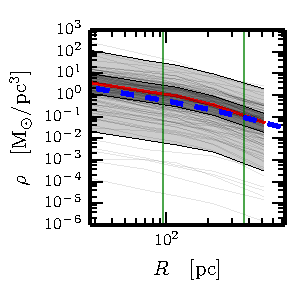
\includegraphics[width=0.4\textwidth]{fig/4_46_201405121422/prof_rho_0}
%        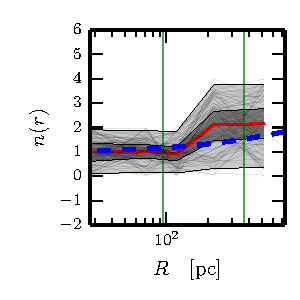
\includegraphics[width=0.4\textwidth]{fig/4_46_201405121422/prof_nr_0}
%        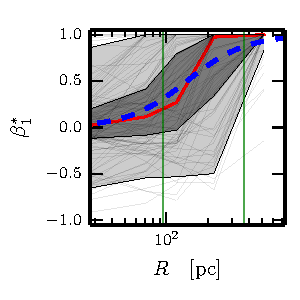
\includegraphics[width=0.4\textwidth]{fig/4_46_201405121422/prof_betastar_1}
%        \includegraphics[width=0.4\textwidth]{fig/4_46_201405121422/prof_betastar_2}
%        \caption{The same cusped profile as in fig. ~\ref{fig:cusp1pop},
%          with $n(r<r_{1/2})<1.5$ prior: Reconstructed mass of the
%          MCMC model (red shows median, shaded areas are 68 and 90
%          percentiles) for all tracer particles. The blue curve shows
%          the underlying theoretical model.}
%        \label{fig:cusp_nr_prior}
%    \end{center}
%\end{figure*}
%
%\begin{figure*}
%    \begin{center}
%        %\hspace{-7mm}
%        % 1-47
%        \includegraphics[width=0.3\textwidth]{fig/1_47_201405060756/prof_rho_0}
%        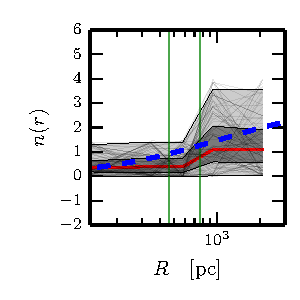
\includegraphics[width=0.3\textwidth]{fig/1_47_201405060756/prof_nr_0}
%        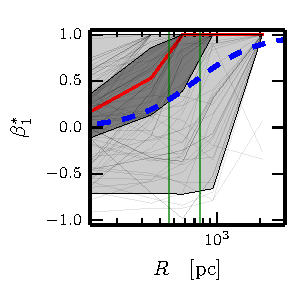
\includegraphics[width=0.3\textwidth]{fig/1_47_201405060756/prof_betastar_1}
%        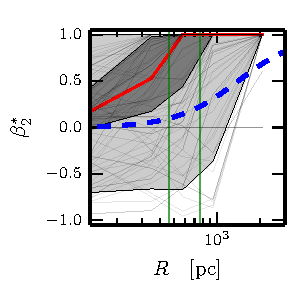
\includegraphics[width=0.3\textwidth]{fig/1_47_201405060756/prof_betastar_2}
%        \caption{The same cored profile as in fig. ~\ref{fig:core2pop},
%          with $n(r<r_{1/2})<1.5$ prior: Reconstructed mass of the
%          MCMC model (red shows median, shaded areas are 68 and 90
%          percentiles) for all tracer particles. The blue curve shows
%          the underlying theoretical model.}
%        \label{fig:core_nr_prior}
%    \end{center}
%\end{figure*}

\subsection{Triaxial mock data}

To test the dependency of \GravImage\ on the
assumption of spherical symmetry, we employ it on
slightly triaxial mock dwarf galaxies.

The models were generated with the Made2Measure
algorithm of \cite{Dehnen2009} and are tailored to
follow a similar profile to the profiles specified
above for the dwarf galaxies. They show a density
profile of

\begin{equation}
    \rho(r)=\frac{\rho_S}{\left(\frac{r}{r_S}\right)^\gamma\left(1+\left(\frac{r}{r_S}\right)^{1/\alpha}\right)^{\alpha(\beta-\gamma)}}
\end{equation}

with radius $r$, scale radius $r_S=1.5\kpc$,
$\alpha=1$, $\beta=4$. For the cusped profiles we
have an inner logarithmic slope of $\gamma=1$,
scale density $\rho_S=5.522\cdot
10^7M_\odot/\kpc^3$, and
$M_{\tot}=1.171\cdot10^9M_\odot$, while for the
cored one we have $\gamma=0.23$,
$\rho_S=1.177\cdot10^8M_\odot$,
$M_{\tot}=1.802\cdot10^9M_\odot$. The axis ratios
are $b/a=0.8$ and $c/a=0.6$. The stars have
negligible mass and follow the same functional
form in the density profile as dark matter, with
$\alpha=0.34, \beta=5.92, \gamma=0.23,
r_S=0.81\kpc$.

The velocity anisotropy of the stellar part is calculated via

\begin{equation}
    \beta(r)=\frac{r_{s,\beta}^\eta \beta_0+r^\eta \beta_\infty}{r^\eta+r_{s,\beta}^\eta},
\end{equation}

with $r_{s,\beta}=0.81\kpc$, $\beta_0=0$, $\beta_\infty=0.5$ and
$\eta=0.5$, going from isotropic to radially anisotropic with
increasing radius.

\begin{figure*}
    \begin{center}
        \hspace{-7mm}
        % triax
        % \includegraphics[width=0.3\textwidth]{fig/Triax01/output/pdf/prof_rho_0.pdf}
        % \includegraphics[width=0.3\textwidth]{fig/Triax01/output/pdf/prof_nr_0.pdf}
        \caption{Density profile of a cusped
          \TODO{triaxial} mock dwarf, for which the line
          of sight is inclined with 45 degrees
          with respect to all axes. The vertical
          line indicates the half-light radius at
          640pc.}
        \label{fig:triax}
    \end{center}
\end{figure*}

The retrieved density profile (fig. \ref{fig:triax}) recaptures the
density inside the half-light radius, but constantly overestimates it
at $r>r_{1/2}$. This is partly due to projection effects, as the
underlying density profile in blue is calculated for spherically
averaged density decrease.

\subsection{Data quality}
How many tracer stars are needed to determine the overall density profile
reliably? To address this question, we performed three runs with a restricted
set of tracer particles. In the first, $10^3$ particles were chosen out of the
$10^6$ simulated particles. With $10^4$ particles, the confidence intervals
shrink. These $10^4$ particles are then split into two populations of each
$5\cdot10^3$ particles, with different scalelengths of $r_S$ and $r_S/10$. Most
of the second population particles are inside the first two bins, so the overall
convergence is not visibly affected above the third bin.  However, the models
are better constrained around the scalelengths of both tracer populations. This
is expected from \citet{WalkerPenarrubia2011}, as any velocity anisotropy
sampling yields the same mass constraint there.

\begin{figure*}
    \begin{center}
        \hspace{-7mm}
        %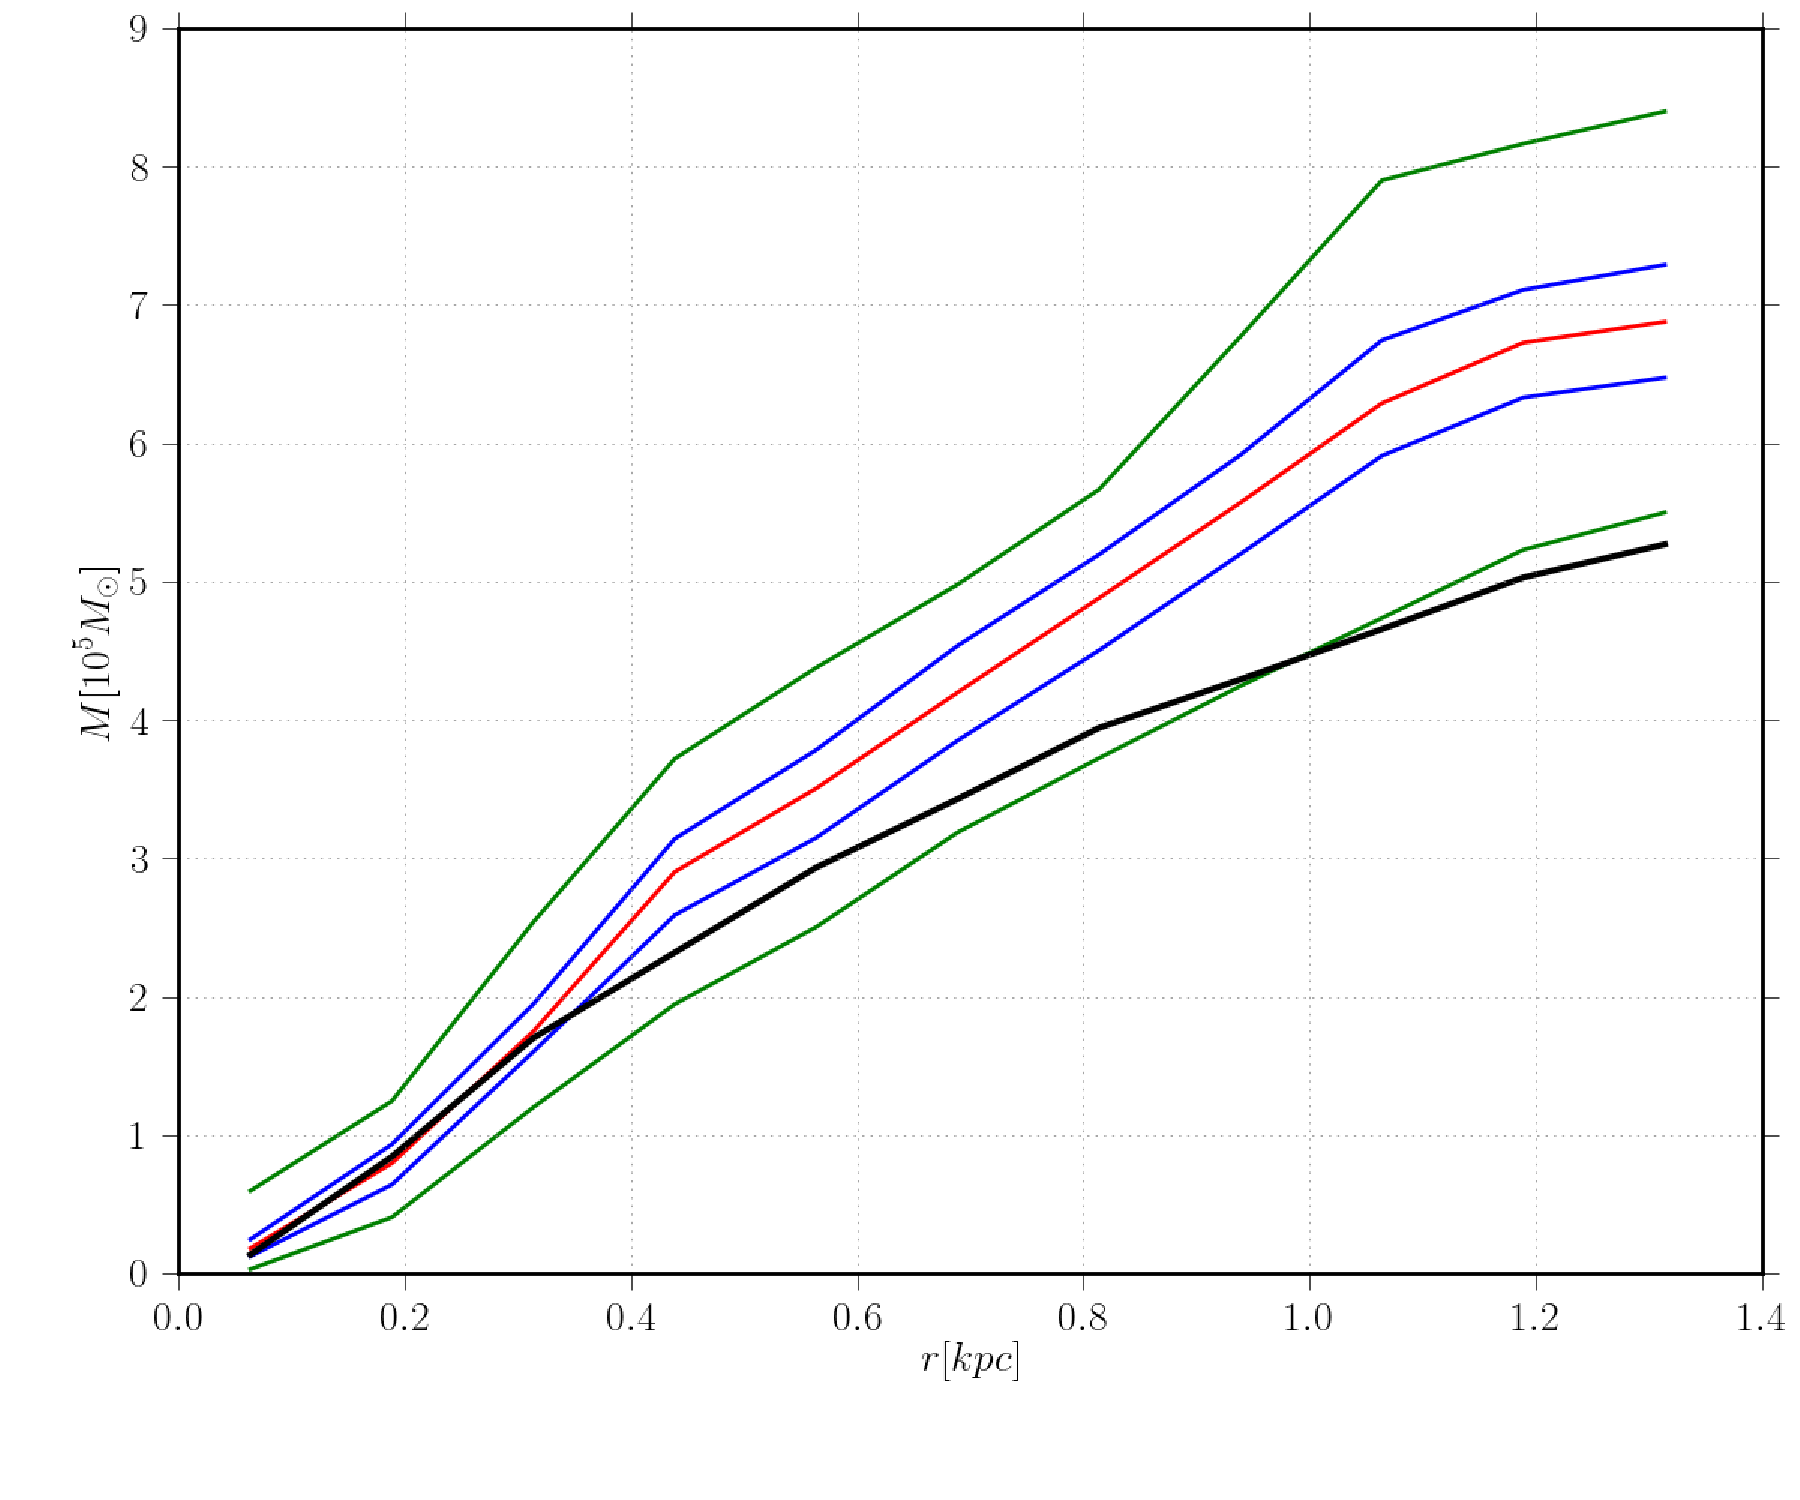
\includegraphics[width=0.3\textwidth]{fig/hernquist1e3.pdf}
        %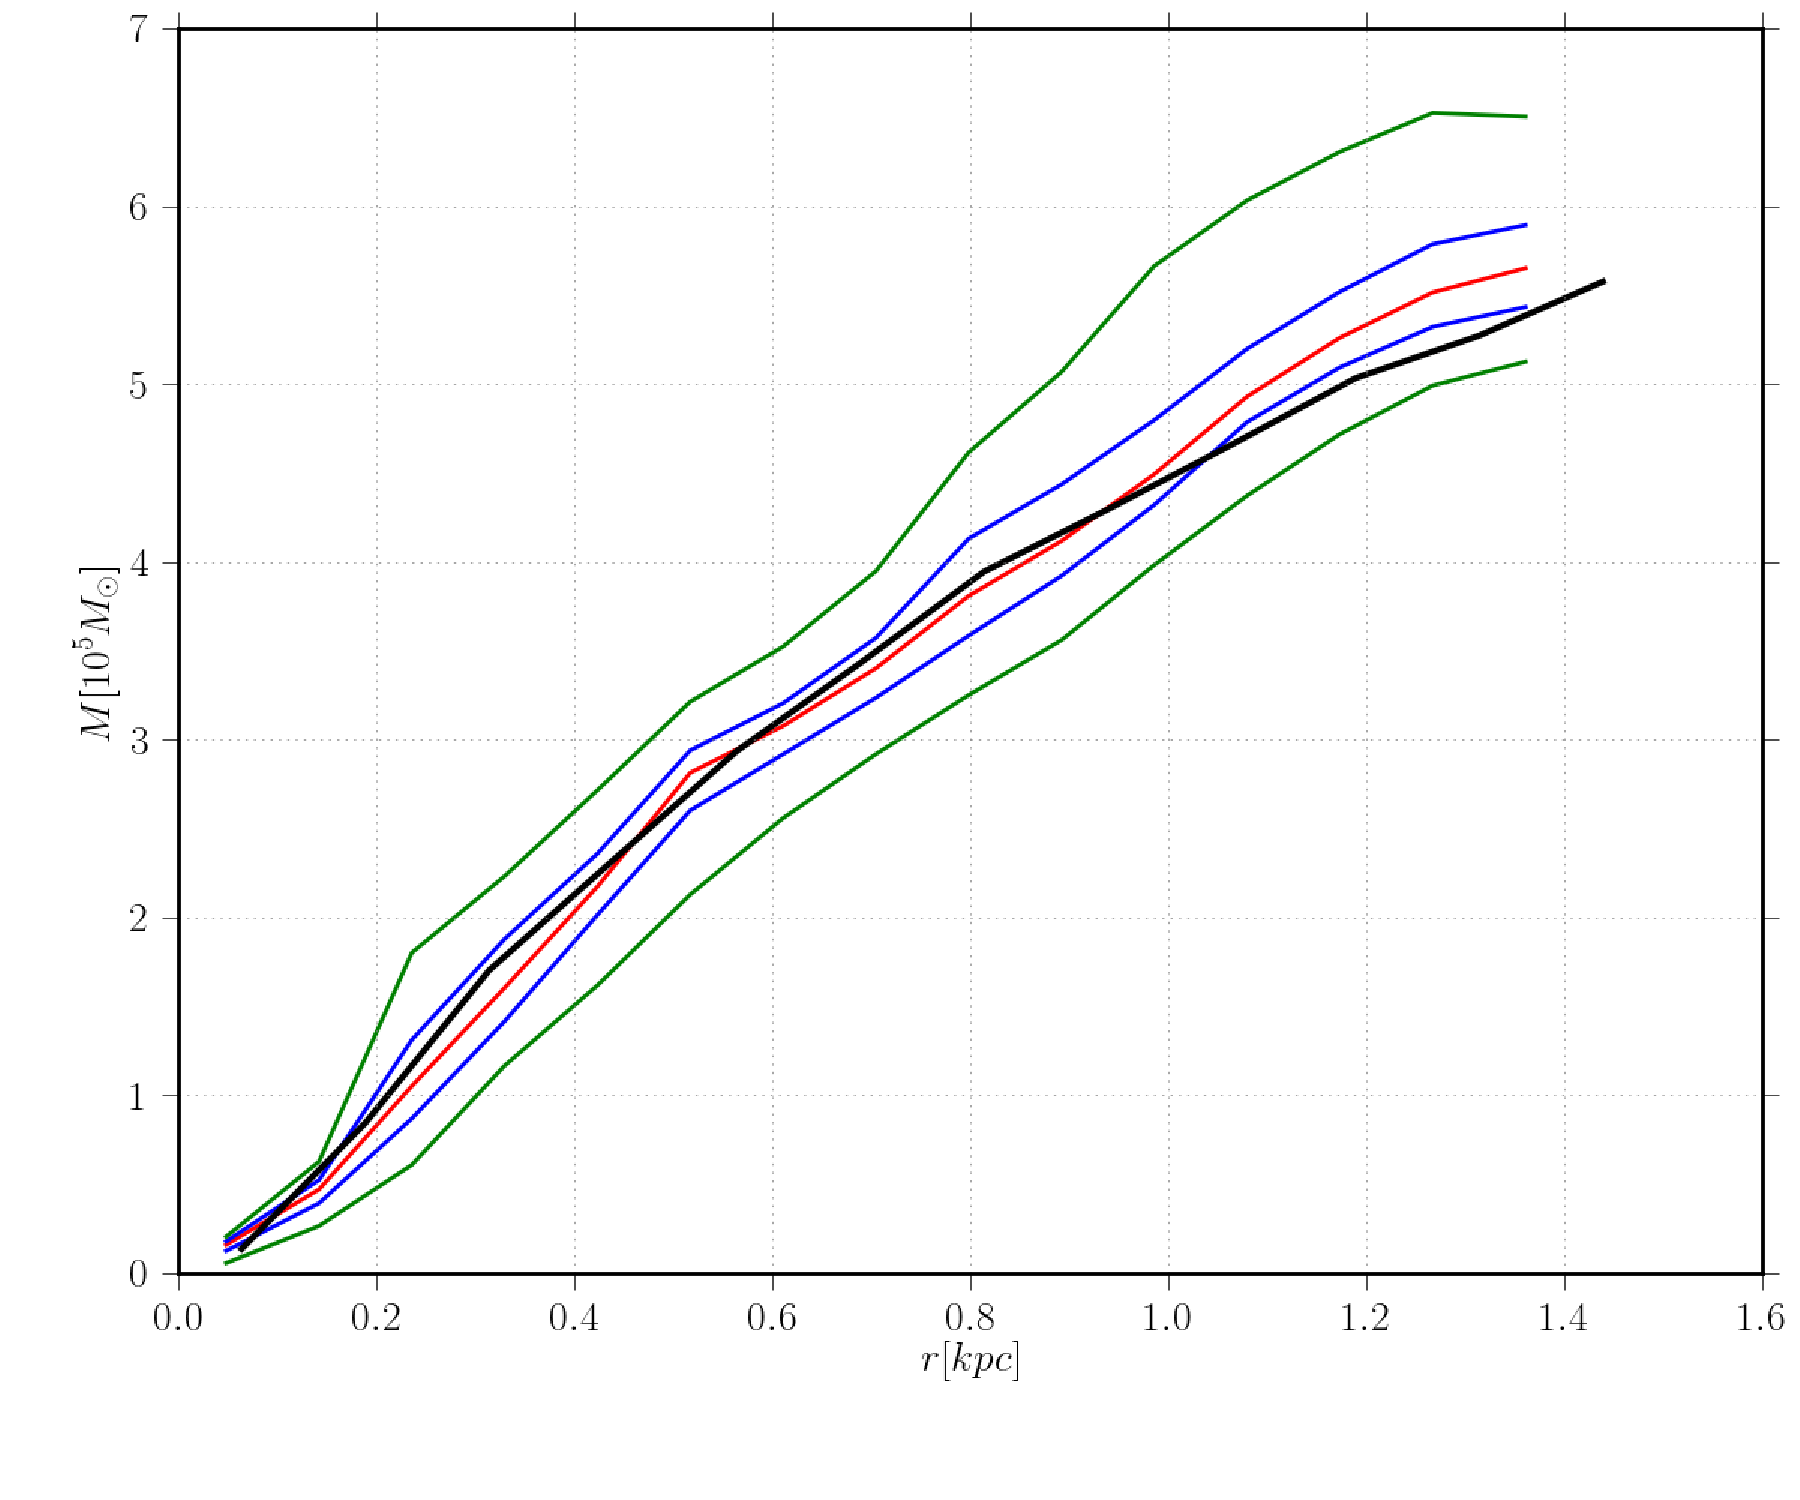
\includegraphics[width=0.3\textwidth]{fig/hernquist1e4.pdf}
        %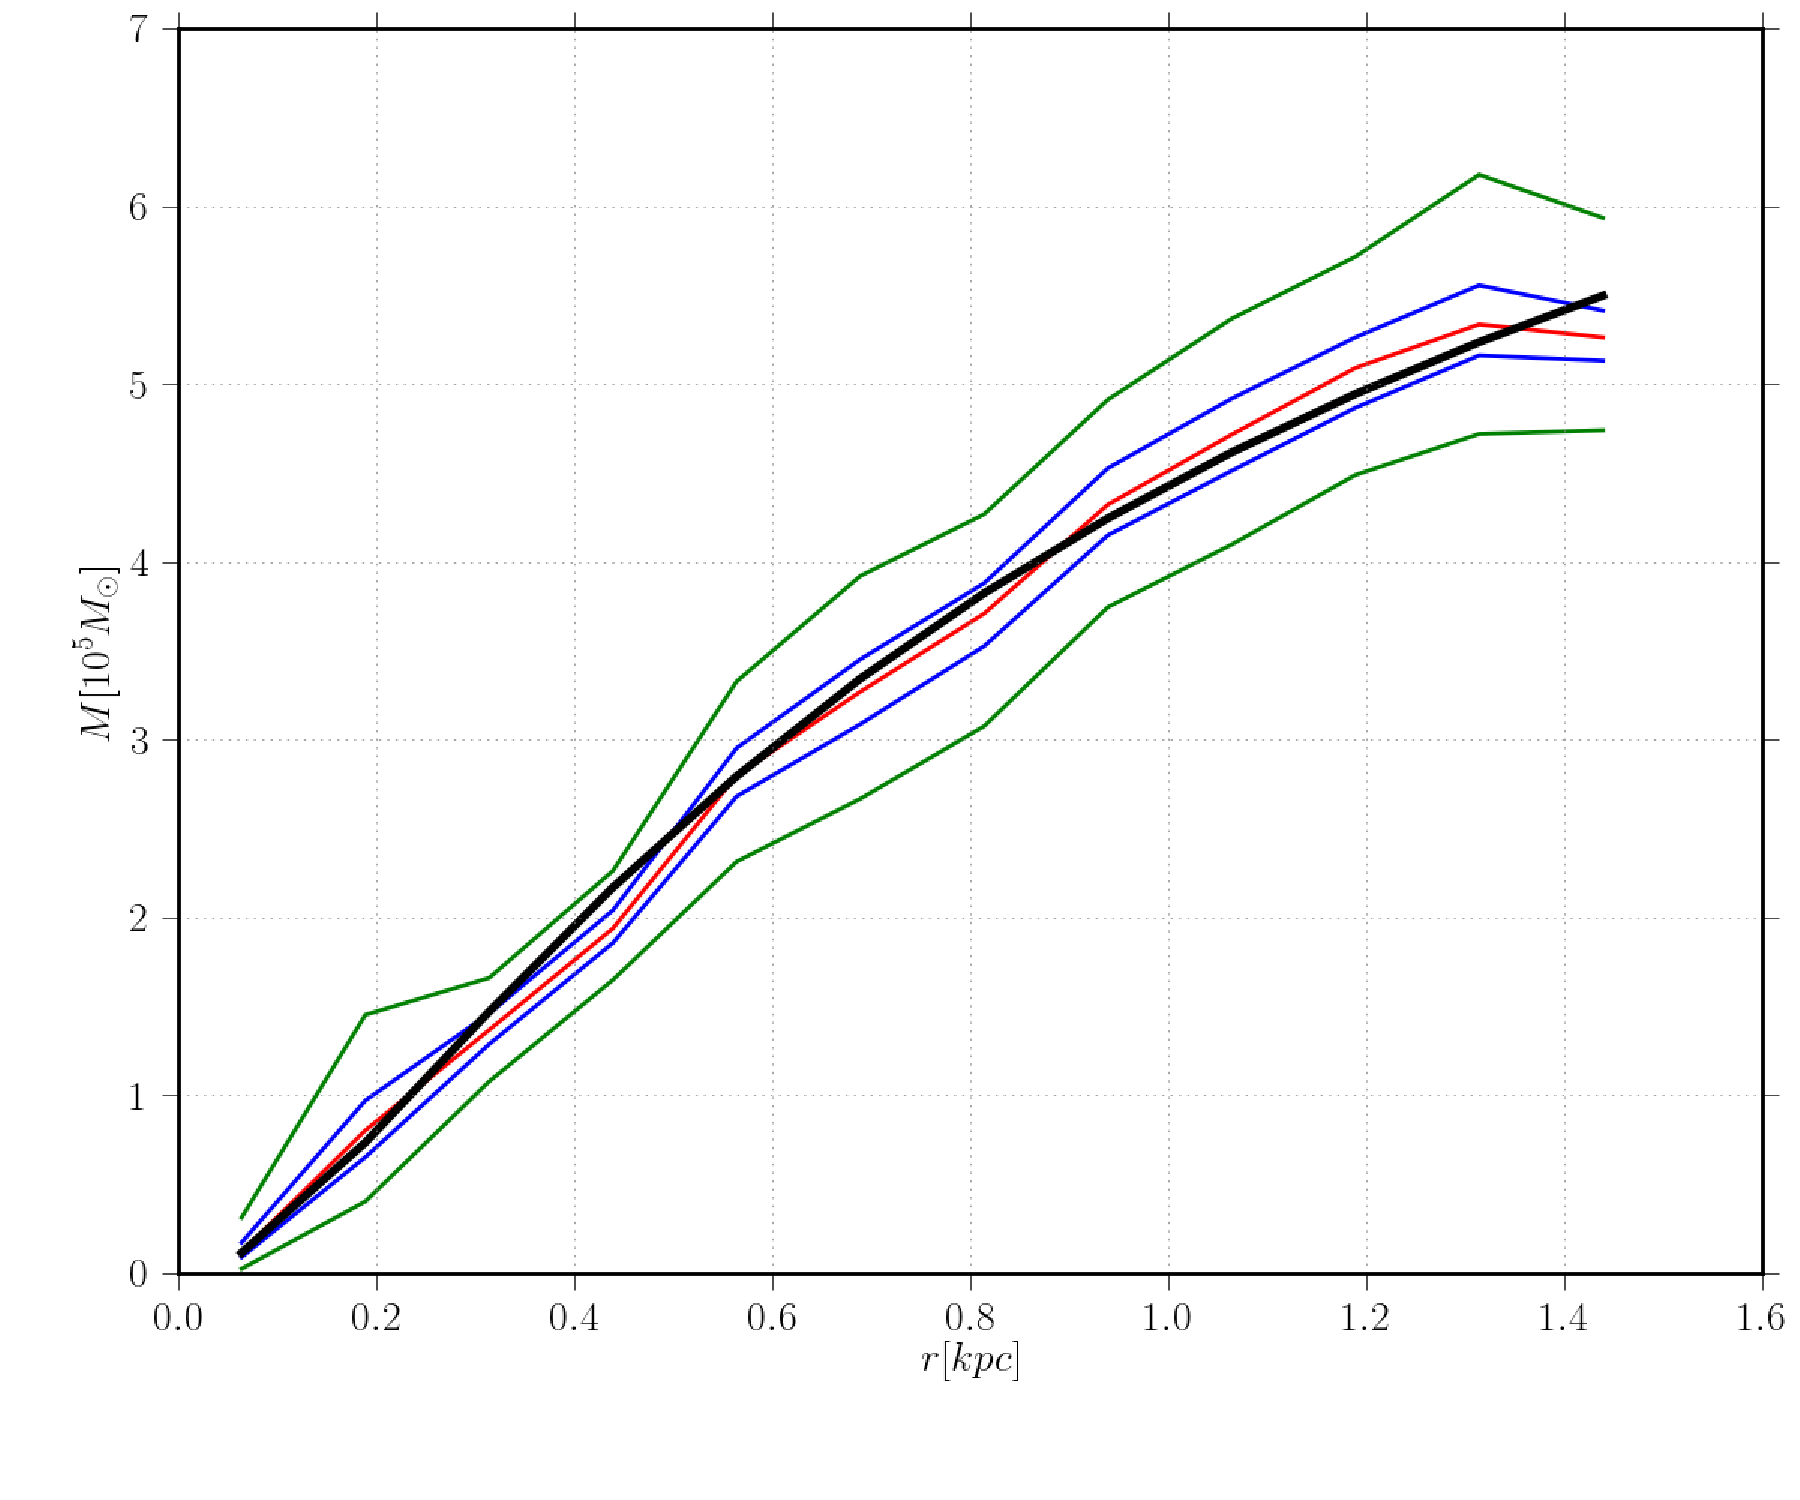
\includegraphics[width=0.3\textwidth]{fig/hernquist2x5e3.pdf}
        \caption{\TODO{Hernquist} profile found by MCMC model (red) for $10^3$,
          $10^4$ and two times $5\cdot10^3$ tracer particles. The black curve
          shows the enclosed mass derived from the theoretical model.}
        \label{fig:hernquist1e3}
    \end{center}
\end{figure*}


%%% Local Variables:
%%% mode: latex
%%% TeX-master: "Steger_2014_GravImage"
%%% End:

\section{Conclusions}\label{sec:conclusions}

\TODO{code reproduces mock data}

\TODO{better with cores/cusp}

\TODO{influences of parameters}

\TODO{minimum data quality needed}

\section{Acknowledgements}
JIR would like to acknowledge support from SNF grant PP00P2\_128540/1.


%%% Local Variables:
%%% mode: latex
%%% TeX-master: "Steger+_2014_GravImage"
%%% End:


\bibliographystyle{mn2e}
\bibliography{Steger+_2014_Gravlite}

%\section{Appendix}

\begin{figure}
    \begin{center}
        %\hspace{-7mm}
        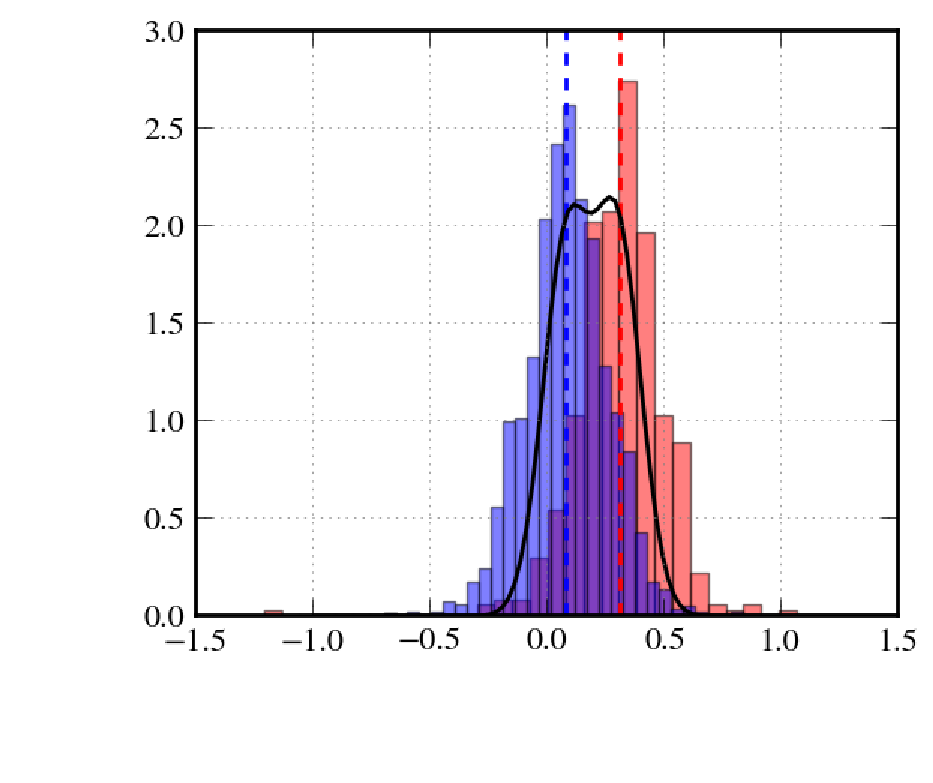
\includegraphics[width=0.5\textwidth]{fig/pymcmetals}
        \caption{Reconstruction of two populations from mock data. The
          underlying metallicity distributions are shown as red and
          blue histograms. The retrieved centers of the Gaussians are
          shown as vertical lines, and the reconstructed metallicity
          distribution is depicted as black line.}
        \label{fig:pymcmetal}
    \end{center}
\end{figure}

%%% Local Variables: 
%%% mode: latex
%%% TeX-master: "Steger+_2014_Gravlite"
%%% End: 


\end{document}
